% !TeX spellcheck = ru_RU
% !TEX root = vkr.tex

\section{Обзор}

Настоящая глава содержит описание реализации многопоточного рантайма tokio, асинхронного интерфейса языка Rust, условий экспериментов.

\subsection{Планировщик многопоточного рантайма tokio}

При инстанциации рантайм создает определенное количество системных потоков для так называемого блокирующего пулла, призванного исполнять ресурсоемкие задачи. Всего создается \verb|worker_threads| + \verb|max_blocking_threads| потоков, где

\begin{itemize}
    \item \verb|worker_threads| --- количество потоков предназначенных для исполнения асинхронных задач
    \item \verb|max_blocking_threads| --- максимальное количество блокирующих потоков
\end{itemize}

\begin{figure}[H]
    \begin{center}
        \makebox[\textwidth]{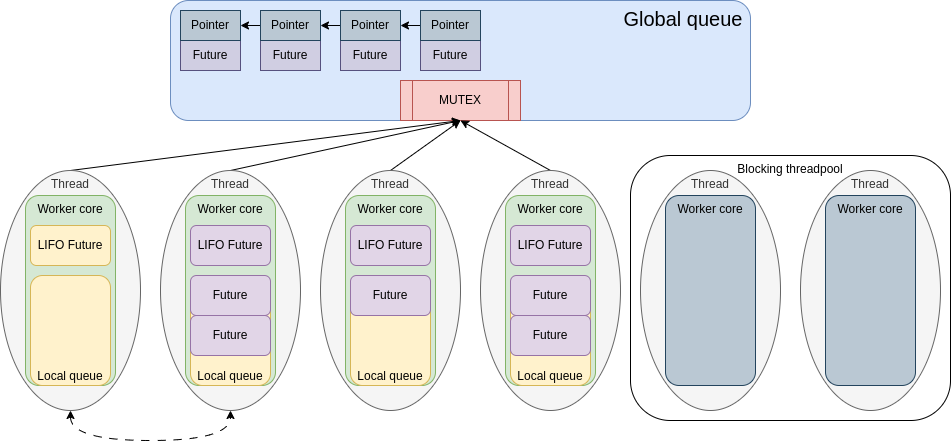
\includegraphics[scale=0.55]{pictures/tokio.arch.png}}
    \end{center}

    \caption{Упрощенное представление многопоточного рантайма}
    \label{fig:tokio:arch}
\end{figure}

\verb|Notified|, так называется тип единицы планирования в tokio. Далее в тексте они также будут называться задачами.

\verb|Воркер|, так называется сущность ассоциированная с каждым из \verb|worker_threads| потоков с помощью размещения в локальной для этих поток переменной так называемого \verb|ядра воркера| --- структуры, необходимой для исполнения асинхронных задач, включающей \verb|локальную очередь|, хендлер \verb|глобальной очереди| и тому подобное.

\verb|Локальная очередь| воркера выступает в качестве кэша задач, имеет фиксированный размер и предполагает добавление элементов  исключительно из потока владельца. Однако, изъятие из нее может быть осуществлено потоками других воркеров при нехватке задач --- процесс называемый похищением. Все это: фиксированный размер и производитель в единственном количестве позволяет ей иметь lock free реализцию. В случае переполнения элементов часть из них перемещается в глобальную очередь.

\verb|Глобальная очередь| или \verb|InjectQueue| представляет собой очередь произвольного размера для агрегации задач. Реализована с помощью интрузивного связного списка, защищенного мьютексом. Именно этот ресурс по мнению разрабочиков из YADRO ограничивает пропускную способность рантайма.

В рамках данной работы будет рассмотрен единственный метод интерфейса планировщика --- \verb|schedule_task|. Именно он используется для отправления на исполнение в планировщик задач. Большое значение имеет контекст вызова этого метода:

\begin{itemize}
    \item В потоке воркера задача будет помещена в его локальную очередь.
    \item В ином случае, задача будет помещена в \verb|InjectQueue|.
\end{itemize}

\subsection{Асинхроное замыкание}

На листинге~\ref{listing:async_closure} представлен код демонстрирующий описание асинхронного замыкания в языке \verb|Rust|.

\begin{listing}[H]
    \begin{minted}{rust}
let closure = async {
    sleep(Duration::from_secs(10)).await;
}
    \end{minted}

    \caption{Асинхронное замыкание}
    \label{listing:async_closure}
\end{listing}

Значениие связанное с именем \verb|closure| представляет собой конечный автомат, имеющий семантику асинхронного ожидания в течении десяти секнуд, сгенерированный компилятором, автоматически реализующий интерфейс представленный на листинге~\ref{listing:future_trait}.

\begin{listing}[H]
    \begin{minted}{rust}
trait Future {
    type Output;
    fn poll(self: Pin<&mut Self>, cx: &mut Context)
        -> Poll<Self::Output>;
}
    \end{minted}

    \caption{Интерфейс асинхронных конечных автоматов в языке Rust}
    \label{listing:future_trait}
\end{listing}

Где метод \verb|poll| выражает попытку совершить переход от состояния к состоянию и сигнализиует о завершении выполнения замыкания с помощью возвращаемого значения типа представленного на листинге~\ref{listing:future:poll}.

\begin{listing}[H]
    \begin{minted}{rust}
enum Poll<T> { Ready(T), Pending }
    \end{minted}

    \caption{Асинхронное замыкание}
    \label{listing:future:poll}
\end{listing}

Способного представить результирующее значение асинхронного вычисления в варианте \verb|Ready| или сигнализировать о отсутствии готового результата с вариантом \verb|Pending|.

Метод \verb|poll| в качестве первого аргумента принимает само асинхронное замыкание, окруженного структурой \verb|Pin| --- это необходимо для статической гарантии безопасности. В качестве второго аргумента --- контекст, служащий оберткой для значния \verb|Waker|.

\subsection{Waker}

Типичным сценарием использования значения \verb|Waker| является:

\begin{itemize}
    \item Создание с помощью специфичной для рантайма таблицы виртуальных методов.
    \item Передача в метод \verb|poll| внутри структуры \verb|Context|.
    \item Если метод poll вернул \verb|Pending| --- замыкание должно зависящим от реализации способом сохранить \verb|Waker| для вызова его метода \verb|wake| при готовности соверщать прогресс.
\end{itemize}

То есть \verb|Waker| является связующим звеном между асинхронным ресурсом и исполнителем асинхронных замыканий, сообщающий первому о готовности второго.

\begin{itemize}
    \item Асинхронный ресурс --- листовые асинхронный замыкания реализованные библиотекой tokio, абстрагирующие архитектурно зависимые интерфейсы, например: epoll, io\_uring, kqueue. TODO(refs)
    \item Исполнитель асинхронных замыканий --- в случае tokio, планировщик, содержащим глобальную очередь.
\end{itemize}

\subsection{Интерфейс tokio}

В следствии выше сказанного любое асинхронное замыкание можно исполнить достатчно долго вызывая на нем метод \verb|poll|, передовая в него \verb|Waker| --- пустышку. Однако, для удобства и эффективности использования асинхронного интерфейса предоставляемого языком \verb|Rust| проект \verb|tokio| предлагает собственный интерфейс для исполнения асинхронных замыканий.

\subsubsection{spawn}

Метод \verb|tokio::spawn| регистрирующий асинхронное замыкание на исполнение в рантайме \verb|tokio| и возвращающий значение \verb|JoinHandle| позволяющее ожидать исполнение исходного замыкания, получить результирующее значение или отменить исполнение вовсе. Например, исполнить представленное выше замыкание можно способом, приведенным на листинге~\ref{listing:tokio_spawn::sleep}:

\begin{listing}[H]
    \begin{minted}{rust}
let join_handle = tokio::spawn(async {
    tokio::time::sleep(Duration::from_secs(10)).await;
})
while !join_handle.is_finished() {}
    \end{minted}

    \caption{Ожидание исполнения асинхронного замыкания}
    \label{listing:tokio_spawn::sleep}
\end{listing}

\subsubsection{yield\_now}

Метод \verb|tokio::task::yeild_now| предоставляет возможность вернуть поток управления планировщику, тем самым создав еще одно состояние в конечном автомате асинхронного замыкания. Его использование приведено на листинге~\ref{listing:tokio_yield_now}.

\begin{listing}[H]
    \begin{minted}{rust}
async {
    task::yield_now().await;
    task::yield_now().await;
}
    \end{minted}

    \caption{Возвращение управления планировщику в tokio}
    \label{listing:tokio_yield_now}
\end{listing}

\verb|yield_now| является листовым асинхронным замыканием, однако никакого настоящего ресурса под собой не содержит. То есть отсутствует внешняя сущность способная уведомить рантайм о готовности замыкания продолжать вычисления --- не кому хранить \verb|Waker|. В подобных случаях для сохранения инстансов типа \verb|Waker| используется локальная для потока воркера коллекция, куда помещается структура \verb|Waker|.

\subsection{Жизненный цикл асинхронного замыкания}

В данном разделе буде описан процесс аллокации асинхронного замыкания и создания первого \verb|Notified| для него.

\subsubsection{Аллокация асинхронного замыкания}

Обработка асинхронного замыкания переданного пользователем в метод \verb|tokio::spawn| содержит следующие шаги:

\begin{itemize}
    \item Создание уникального индентификатора. Просиходит это с помощью статической атомарной переменной над которой выполняется FAA с relaxed семантикой.
    \item Аллокации структуры содержащей замыкание, счетчик указателей, слот для результирующего значения и тому подобных --- так называемой \verb|Cell| на куче.
    \item Созданием трех указатейлей на эту область памяти: \verb|Task|, \verb|Notified| и \verb|JoinHandle|.
    \begin{itemize}
        \item \verb|Task| помещается в \verb|OwnedTasks| --- очередь, предназначенную для хранения указателей на все замыкания исполняемые рантаймом.
        \item \verb|Notified| является единицей планирования и отправляется в планировщик c помощью метода \verb|schedule_task|.
        \item \verb|JoinHandle| возвращается пользователю.
    \end{itemize}
\end{itemize}

\subsubsection{Исполнение замыкания}

Далее, происходит исполнения замыкания: после вызова метода \verb|wake| у соотвествующего инстанса типа \verb|Waker|, новый указатель \verb|Notified| отправляется в планировщик \verb|tokio| рантайма c помощью метода \verb|schedule_task|. Далее у \verb|Notified| будет вызван метод \verb|poll|, что повлечет исполнение метода \verb|poll| на исходном замыкании.

Таким образом по готовности каждого асинхронного замыкания уже аллоцированного tokio рантаймом создается указатель \verb|Notified| отправляемый на исполнение в планировщик с \verb|schedule_task|.

\subsubsection{Удаление замыкания}

При достижении конечного состояни \verb|Task| удаляется из \verb|OwnedTasks|, \verb|Cell| деаллоцируется.

\subsubsection{Цикл работы воркера}

После сказанного выше следует рассмотреть упрощенный цикл работы вокрера отраженный на листинге~\ref{listing:worker:run}.

\begin{listing}[H]
    \begin{minted}{rust}
loop {
    worker.tick();
    if let Some(task) = worker.next_task() {
        worker.run_task(task);
        continue;
    }
    if let Some(task) = worker.steal_work() {
        worker.run_task(task);
        continue;
    }
    if !worker.wakers.is_empty() {
        worker.wakers.wake();
        continue;
    }
    worker.park();
}
    \end{minted}

    \caption{Логика выбора следующей задачи}
    \label{listing:worker:run}
\end{listing}

А именно:

\begin{itemize}
    \item Воркер отсчитывает тик --- единицу времени воркера.
    \item Затем пытается найти задачу в локальной, затем в глобальной очереди.
    \item После чего пытается украсть задачи у других воркеров.
    \item Вызывает метод \verb|wake| на всех задачах зарегистрировавших структуру \verb|Waker| в потоке воркера. То есть отправляет на исполнение с помощью \verb|schedule_task| структуры \verb|Notified| для задач совершивших \verb|yield_now| в потоке воркера, тем самым насыщая локальную очередь задачами, и снова пытается найти задачу.
    \item Если очереди оказываются пустыми паркует поток.
\end{itemize}

Заполучив структуру \verb|Notified| воркер вызовет на ней один раз метод \verb|poll|.

\subsection{Условия экспериментов}

Для измерений производительности была использована библиотека \verb|criterion|\footnote{\href{https://github.com/bheisler/criterion.rs}{Репозиторий} проекта criterion (Дата обращения: 4.1.2025)}. Так как она популярна, имеет обширную документацию и используется в \verb|tokio|.

Здесь и далее эксперименты производились при следующих условиях:

\begin{itemize}
    \item Исследования проводились на системе YADRO VEGMAN Rx20 G2\footnote{\href{https://yadro.com/ru/vegman/rx20g2/specs}{Описание} системы YADRO VEGMAN Rx20 G2}.
    \item Бенчмарк был запущен с значением \verb|nice| равным минус двадцати.
    \item Исполнение было рекомендовано на одной NUMA единице с помощью \verb|taskset|.
\end{itemize}

Машина для измерение производительности была любезно предоставлена командой \verb|TATLIN.BACKUP| и находилась удаленно, в связи с чем на ней было невозможно отключение сети.

Библиотека criterion сконфигурирована следующим образом:

\begin{itemize}
    \item Пять секунд прогрева.
    \item Сорок семплов для каждого измерения.
    \item Линеаризация в качестве способа семплирования.
\end{itemize}
